\clearpage
\appendix

\section{Dataset: MATH-100-multi}
\label{app:dataset}

This section describes the MATH-100-multi dataset, including the construction prompts used to decompose MATH-500 problems into multi-turn sequences, and the resulting turn-count distribution.

\subsection{Decomposition Prompts}
\label{app:decompose_prompt}

The following prompts were used to construct the MATH-100-multi dataset, including the System Prompt and User Template.

\subsubsection*{System Prompt}

\begin{small}
\begin{lstlisting}[basicstyle=\ttfamily\footnotesize, breaklines=true, breakatwhitespace=false, columns=flexible, keepspaces=true]
You are a math problem decomposer. Your sole
task is to decompose a given math problem into
a multi-turn QA sequence that simulates a
teacher guiding a student step by step.

### Decomposition Rules

1. **Determine n automatically** based on
   solution complexity:
   - 1-2 key computation steps -> n = 2
   - 3-4 key computation steps -> n = 3~4
   - 5+ steps or multi-concept problems
     -> n = 4~6
   - Never inflate n with trivial or
     redundant sub-questions.

2. **Strict numerical carry-over dependency**:
   - Each q_i (i >= 2) must explicitly
     reference the numerical result produced
     by q_{i-1}.
   - Phrase q_i so the dependency is visible
     in the question text itself, e.g.:
     "Using the value of X you found in the
     previous step, ..."
   - A sub-question that can be answered
     without the prior numerical result is
     invalid.

3. **Coverage and chain completeness**:
   - The sub-questions q1 -> q2 -> ... -> qn
     must form a COMPLETE and CONTINUOUS
     reasoning chain that leads to the final
     answer.
   - The final answer must emerge from the
     chain naturally -- it must NEVER be
     injected into qn without derivation.
   - q_n must be the step that directly
     produces the final answer through
     reasoning, not a step that merely
     states it.

4. **Naturalness**: Sub-questions should read
   as genuine interrogative prompts, not
   restatements of solution steps.

5. **Answer generation**:
   - Each a_i must directly answer q_i as if
     a student is solving it from scratch --
     show the actual computation or derivation
     steps, do NOT merely state the conclusion.
   - Use the provided Solution as a reference
     to ensure correctness, but write each
     answer in the student's own working style:
       correct: "d/60 + d/40 = (2d+3d)/120
                = 5d/120 = 5, so d = 120 km."
       wrong:   "The distance is 120 km."
                (conclusion only)
   - a_i must include the specific numerical
     result that q_{i+1} will depend on,
     stated clearly at the end, e.g.:
     "Therefore, d = 120 km."
   - a_n must match the original problem's
     final Answer exactly.
   - WARNING: If a_n cannot be reached
     naturally from a_{n-1}, the
     decomposition is broken. Restructure
     from q1 -- do NOT patch qn to force
     the answer.

6. **Solution invisibility**:
   - The provided Solution is for YOUR
     reference only to understand the
     problem structure.
   - NEVER mention, quote, or reference the
     Solution in any question or answer.
   - Questions and answers must read as if
     the Solution does not exist.

### Output Format
Return **only** a valid JSON object. No
explanation, no markdown, no text outside
the JSON.

{
  "turns": <n>,
  "qa_pairs": [
    {"question": "q1: ...",
     "answer": "a1: ..."},
    {"question": "q2: ... (using the result
                  X from q1, ...)",
     "answer": "a2: ..."},
    ...
    {"question": "qn: ...",
     "answer": "an: ..."}
  ]
}
\end{lstlisting}
\end{small}

\subsubsection*{User Template}

\begin{small}
\begin{lstlisting}[basicstyle=\ttfamily\footnotesize, breaklines=true, breakatwhitespace=false, columns=flexible, keepspaces=true]
Please decompose the following math problem
into a multi-turn question sequence.

### Problem
{problem}

### Solution
{solution}

### Answer
{answer}
\end{lstlisting}
\end{small}

\noindent where \verb|{problem}|, \verb|{solution}|, and \verb|{answer}| are replaced with the corresponding entries from the MATH-500 dataset.

\subsection{Turn-Count Distribution}
\label{app:turn_dist}

Table~\ref{tab:turn_dist} shows the distribution of sub-question counts across the 100 problems in the MATH-100-multi dataset, as determined by the decomposition pipeline.

\begin{table}[h]
\centering
\begin{tabular}{ccc}
\toprule
\textbf{Turns} & \textbf{Count} & \textbf{Percentage} \\
\midrule
2 & 13 & 13.0\% \\
3 & 58 & 58.0\% \\
4 & 26 & 26.0\% \\
5 &  3 &  3.0\% \\
\midrule
Total & 100 & 100.0\% \\
\bottomrule
\end{tabular}
\caption{Turn-count distribution of MATH-100-multi ($n=100$).}
\label{tab:turn_dist}
\end{table}

%% ----------------------------------------------------------------
\section{Prompts}
\label{app:prompts}

This section provides the complete prompts used by Agent~$\mathcal{B}$ and the LLM judge.

\subsection{Agent B: Extract Step}
\label{app:agent_b_prompt}

\begin{lstlisting}[basicstyle=\small\ttfamily, breaklines=true, frame=none, xleftmargin=0.5em, xrightmargin=0.5em]
You are a mathematical knowledge extractor. Given a reasoning
response to a math sub-question, extract the key logical
propositions that represent concrete mathematical claims.

A valid proposition is one of:
- An equation or inequality: "x = 3", "n >= 2"
- A specific numeric result: "The answer is 42"
- A named property: "n is prime", "f is injective on [0,1]"

Rules:
- Each proposition must be self-contained and atomic.
- Write it as a direct claim, not a description of a step.
- Omit reasoning steps that are not reusable facts.

NEVER extract:
- Section headers like "Step 1:", "Setup:"
- Definitions that describe what a term means
- Process descriptions like "We simplify..."
- Bold phrases describing what you are about to do

Your response must contain EXACTLY this structure:
FINAL_LIST_START
1. <proposition>
2. <proposition>
FINAL_LIST_END
\end{lstlisting}

\subsection{Agent B: Merge Step}

\begin{lstlisting}[basicstyle=\small\ttfamily, breaklines=true, frame=none, xleftmargin=0.5em, xrightmargin=0.5em]
You are a mathematical knowledge base curator. Given an existing
list of facts and a list of new propositions, output the merged,
deduplicated list of mathematical facts.

Rules:
- Drop any new proposition already covered by an existing fact.
- Drop any existing fact superseded or contradicted by a new
  proposition (keep the new one instead).
- Keep all remaining facts combined.
- Do NOT write any analysis, reasoning, or commentary.

Your response must contain EXACTLY this structure:
FINAL_LIST_START
1. <fact>
2. <fact>
FINAL_LIST_END
\end{lstlisting}

\subsection{LLM Judge}
\label{app:judge_prompt}

The complete prompts used by the LLM judge (Kimi K2.6) for per-turn accuracy (ACC) evaluation. The judge receives all sub-questions for a problem in a single structured call and outputs verdicts simultaneously.

\subsubsection*{System Prompt}

\begin{lstlisting}[basicstyle=\small\ttfamily, breaklines=true, frame=none, xleftmargin=0.5em, xrightmargin=0.5em]
You are a rigorous mathematical evaluator for a multi-turn reasoning
system. You will be given a math problem decomposed into ordered
sub-questions. For each sub-question, you must judge whether the
model's answer is correct by comparing it against the gold reference
answer.

# Evaluation Criteria

For each turn, assign one of three verdicts:

- "correct": The model reaches the same mathematical conclusion as
  the gold answer. Different notation, variable names, or derivation
  paths are acceptable as long as the final stated result is
  mathematically equivalent.
- "partially_correct": The model demonstrates correct understanding
  of the approach but makes algebraic/computational errors, OR
  reaches a result that captures part but not all of the gold
  conclusion.
- "incorrect": The model's final conclusion contradicts the gold
  answer, fails to produce a usable conclusion, or answers a
  different question.

# Important Rules

1. Judge each turn independently. Do NOT penalize a later turn for
   using a value that contradicts an earlier (wrong) turn's output
   -- evaluate only whether the current turn's conclusion matches
   its own gold answer.
2. Focus on the FINAL stated conclusion of the model, not
   intermediate scratch work. Verbosity is not a defect.
3. Mathematical equivalence over textual similarity. `c = -2` and
   `the coefficient equals -2` are the same.
4. If the model fails to reach a conclusion (e.g., trails off, gets
   stuck mid-derivation), mark it `incorrect`.
5. Notation drift: if the model invents new variables (e.g., `c_1`
   vs `c`) but the conclusion is still equivalent, treat as correct.

# Output Format

Return ONLY a valid JSON object, no preamble, no markdown fences:

{
  "evaluations": [
    {
      "turn": <int>,
      "verdict": "correct" | "partially_correct" | "incorrect",
      "model_conclusion": "<one-line summary of what the model
                           actually concluded for this sub-question>",
      "gold_conclusion": "<one-line summary of the gold answer's
                          conclusion>",
      "rationale": "<1-2 sentences explaining the verdict, citing
                    the specific discrepancy if any>"
    }
  ],
  "num_correct": <int>,
  "num_partial": <int>,
  "num_incorrect": <int>,
  "overall_summary": "<2-3 sentences on the model's reasoning
                      pattern across turns>"
}
\end{lstlisting}

\subsubsection*{User Template}

Each call assembles the user message from the following template, where \texttt{\{problem\}} is the problem text, \texttt{\{gold\_final\_answer\}} is the final reference answer, and \texttt{\{turns\_block\}} is a concatenation of per-turn blocks each containing \texttt{sub\_question}, \texttt{gold\_answer}, and \texttt{model\_answer}.

\begin{lstlisting}[basicstyle=\small\ttfamily, breaklines=true, frame=none, xleftmargin=0.5em, xrightmargin=0.5em]
<main_problem>
{problem}
</main_problem>

<gold_final_answer>
{gold_final_answer}
</gold_final_answer>

<turns>
<turn id="{turn_id}">
  <sub_question>{question}</sub_question>
  <gold_answer>{gold_answer}</gold_answer>
  <model_answer>{model_answer}</model_answer>
</turn>
...
</turns>
\end{lstlisting}

%% ----------------------------------------------------------------
\section{Implementation Details}
\label{app:implementation}

All models are served using vLLM with \texttt{enable\_thinking=True} to activate the extended reasoning mode of Qwen3.5 models. Inference uses greedy decoding: temperature~$= 0$, top-$p = 1.0$, and \texttt{max\_tokens}~$= 16{,}384$. Each sub-question is issued as a fresh single-turn call; no multi-turn chat history is passed to the model API directly---state is managed externally by the compression strategies. Agent~$\mathcal{B}$ (curator) calls use the same vLLM instance with \texttt{max\_tokens}~$= 512$. The LLM judge (Kimi~K2.6) is called via its public API with \texttt{temperature}~$= 0$.

%% ----------------------------------------------------------------
\section{Extended Experimental Results}
\label{app:results}

This section provides extended experimental results not included in the main paper due to space constraints.

\subsection{Failure Mode Analysis: Full History at 4B}
\label{app:fh_failure}

Table~\ref{tab:fh_failure} reports the failure mode distribution for 31 problems where Full History fails but at least one compression method achieves higher per-turn accuracy at the Qwen3.5-4B scale.

\begin{table}[h]
\centering
\small
\caption{Failure mode distribution of Full History on Qwen3.5-4B (31 problems where compression methods achieve higher per-turn accuracy). Categories are not mutually exclusive; rows may sum to $>$100\%.}
\label{tab:fh_failure}
\begin{tabular}{lrr}
  \toprule
  \textbf{Failure mode} & \textbf{Count} & \textbf{\%} \\
  \midrule
  Response-style cascade                   & 7  & 22.6 \\
  Answer truncation at \texttt{max\_tokens} & 23 & 74.2 \\
  Numerical condition forgetting           & 1  &  3.2 \\
  Logic error unrelated to context         & 0  &  0.0 \\
  Other                                    & 0  &  0.0 \\
  \bottomrule
\end{tabular}
\end{table}

\subsection{Failure Mode Analysis: Compression at 2B}
\label{app:slsc_failure}

Table~\ref{tab:slsc_failure} reports the failure mode distribution for 16 problems where compression methods fail but Full History succeeds at the Qwen3.5-2B scale.

\begin{table}[h]
\centering
\small
\caption{Failure mode distribution of compression methods on Qwen3.5-2B (16 problems where Full History succeeds, compression fails).}
\label{tab:slsc_failure}
\begin{tabular}{lrr}
  \toprule
  \textbf{Failure mode} & \textbf{Count} & \textbf{\%} \\
  \midrule
  Fails to parse compressed representation & 0  &  0.0 \\
  Ignores state, re-derives from $P$       & 2  & 12.5 \\
  Misinterprets state semantics            & 13 & 81.3 \\
  Other                                    & 1  &  6.3 \\
  \bottomrule
\end{tabular}
\end{table}

\subsection{Correct Turn Rate Across All Scales}
\label{app:ctr_full}

Table~\ref{tab:ctr_full} reports the Correct Turn Rate (CTR) --- the fraction of individual sub-question turns answered correctly --- across all four model scales. While the main paper (Table~\ref{tab:main}) focuses on Fully Correct Rate (FCR), CTR provides a finer-grained view of per-turn performance.

\begin{table}[h]
\centering
\small
\setlength{\tabcolsep}{4pt}
\begin{tabular}{lcccc}
\toprule
\textbf{Reasoner} & \textbf{No Comp.} & \textbf{Sum.} & \textbf{SLSC\,w/o} & \textbf{SLSC} \\
\midrule
Qwen3.5-0.8B & 23.2 & 40.5 & 45.8 & 44.2 \\
Qwen3.5-2B   & 69.6 & 70.2 & 69.3 & 67.1 \\
Qwen3.5-4B   & 80.6 & 86.5 & 86.5 & 85.9 \\
Qwen3.5-9B   & 81.2 & 90.3 & 91.8 & 90.3 \\
\bottomrule
\end{tabular}
\caption{CTR (\%, higher is better) across all model scales. ``Sum.''~= Summary; ``SLSC\,w/o''~= SLSC without Lean~4.}
\label{tab:ctr_full}
\end{table}

\subsection{Token Usage Across All Scales}
\label{app:tokens_full}

Table~\ref{tab:tokens_full} extends the token analysis from the main paper (Table~\ref{tab:tokens}, which covers 4B only) to all four model scales. The ``Saving'' columns report reduction in per-turn input tokens relative to the No Compression baseline.

\begin{table}[h]
\centering
\small
\resizebox{\columnwidth}{!}{%
\begin{tabular}{lrrrrccc}
\toprule
 & \multicolumn{4}{c}{\textbf{Avg.\ tokens / turn}} & \multicolumn{3}{c}{\textbf{Saving vs.\ No Comp.}} \\
\cmidrule(lr){2-5}\cmidrule(lr){6-8}
\textbf{Model} & \textbf{No Comp.} & \textbf{Summary} & \textbf{SLSC w/o F.} & \textbf{SLSC} & \textbf{Summary} & \textbf{SLSC w/o F.} & \textbf{SLSC} \\
\midrule
Qwen3.5-0.8B & 4509 & 768 & 913 & 1533 & 83.0\% & 79.8\% & 66.0\% \\
Qwen3.5-2B   & 3864 & 766 & 862 & 1332 & 80.2\% & 77.7\% & 65.5\% \\
Qwen3.5-4B   & 3058 & 766 & 806 & 1153 & 74.9\% & 73.6\% & 62.3\% \\
Qwen3.5-9B   & 2767 & 765 & 821 & 1205 & 72.4\% & 70.3\% & 56.4\% \\
\bottomrule
\end{tabular}%
}
\caption{Average per-turn input tokens and percentage savings across all model scales. ``No Comp.'' = No Compression; ``Summary'' = Natural-Language Summary; ``SLSC w/o F.'' = SLSC without Lean~4; ``SLSC'' = SLSC with Lean~4.}
\label{tab:tokens_full}
\end{table}

\subsection{Per-Turn Accuracy at Qwen3.5-4B}
\label{app:per_turn_4b}

Table~\ref{tab:per_turn_4b} reports the per-turn CTR at the 4B scale with the sample size $n$ at each turn position. Turn~5 has only 3 problems and should be interpreted with caution. The figure in the main paper (Figure~\ref{fig:per_turn}) visualizes similar trends across all scales; this table adds exact values and sample sizes for the focal 4B model.

\begin{table}[h]
\centering
\small
\setlength{\tabcolsep}{4pt}
\begin{tabular}{ccccc r}
\toprule
\textbf{Turn} & \textbf{No Comp.} & \textbf{Sum.} & \textbf{SLSC w/o} & \textbf{SLSC} & \textbf{$n$} \\
\midrule
1 & 84.0 & 91.0 & 91.0 & 91.0 & 100 \\
2 & 81.0 & 88.0 & 85.0 & 83.0 & 100 \\
3 & 80.5 & 87.4 & 87.4 & 87.4 &  87 \\
4 & 69.0 & 69.0 & 75.9 & 75.9 &  29 \\
5 & 66.7 & 33.3 & 66.7 & 66.7 &   3 \\
\bottomrule
\end{tabular}
\caption{Per-turn CTR (\%) at Qwen3.5-4B. ``Sum.'' = Summary; ``SLSC w/o'' = SLSC without Lean~4. $n$ = number of problems with at least that many turns.}
\label{tab:per_turn_4b}
\end{table}

\subsection{Category-Level Correct Turn Rate}
\label{app:category}

Table~\ref{tab:category_ctr} shows CTR broken down by the seven subject categories in the MATH-500 benchmark. Results are averaged across all four model scales to give a category-level view of where each compression strategy provides the most benefit.

\begin{table}[h]
\centering
\footnotesize
\setlength{\tabcolsep}{3pt}
\begin{tabular}{lcccc}
\toprule
\textbf{Category} & \textbf{No C.} & \textbf{Sum.} & \textbf{SLSC\,w/o} & \textbf{SLSC} \\
\midrule
Algebra              & 72.3 & 77.8 & 78.5 & 77.1 \\
Counting \& Prob.    & 57.0 & 65.4 & 67.2 & 65.8 \\
Geometry             & 55.2 & 63.1 & 63.8 & 62.4 \\
Interm.\ Algebra     & 58.6 & 67.3 & 68.9 & 67.5 \\
Number Theory        & 62.4 & 73.2 & 76.1 & 74.8 \\
Prealgebra           & 78.9 & 81.4 & 82.0 & 80.6 \\
Precalculus          & 53.7 & 62.9 & 65.3 & 63.7 \\
\midrule
\textbf{Overall}     & \textbf{63.7} & \textbf{70.2} & \textbf{71.7} & \textbf{70.3} \\
\bottomrule
\end{tabular}
\caption{CTR (\%) by MATH subject category, averaged across all four model scales. ``No C.''~= No Compression; ``Sum.''~= Summary; ``SLSC\,w/o''~= SLSC without Lean~4.}
\label{tab:category_ctr}
\end{table}

\subsection{Verdict Distribution Across Conditions}
\label{app:verdict_dist}

Figure~\ref{fig:verdict_dist} shows the breakdown of per-turn verdicts (correct, partially correct, incorrect) for each compression condition across all four model scales.

\begin{figure*}[t]
\centering
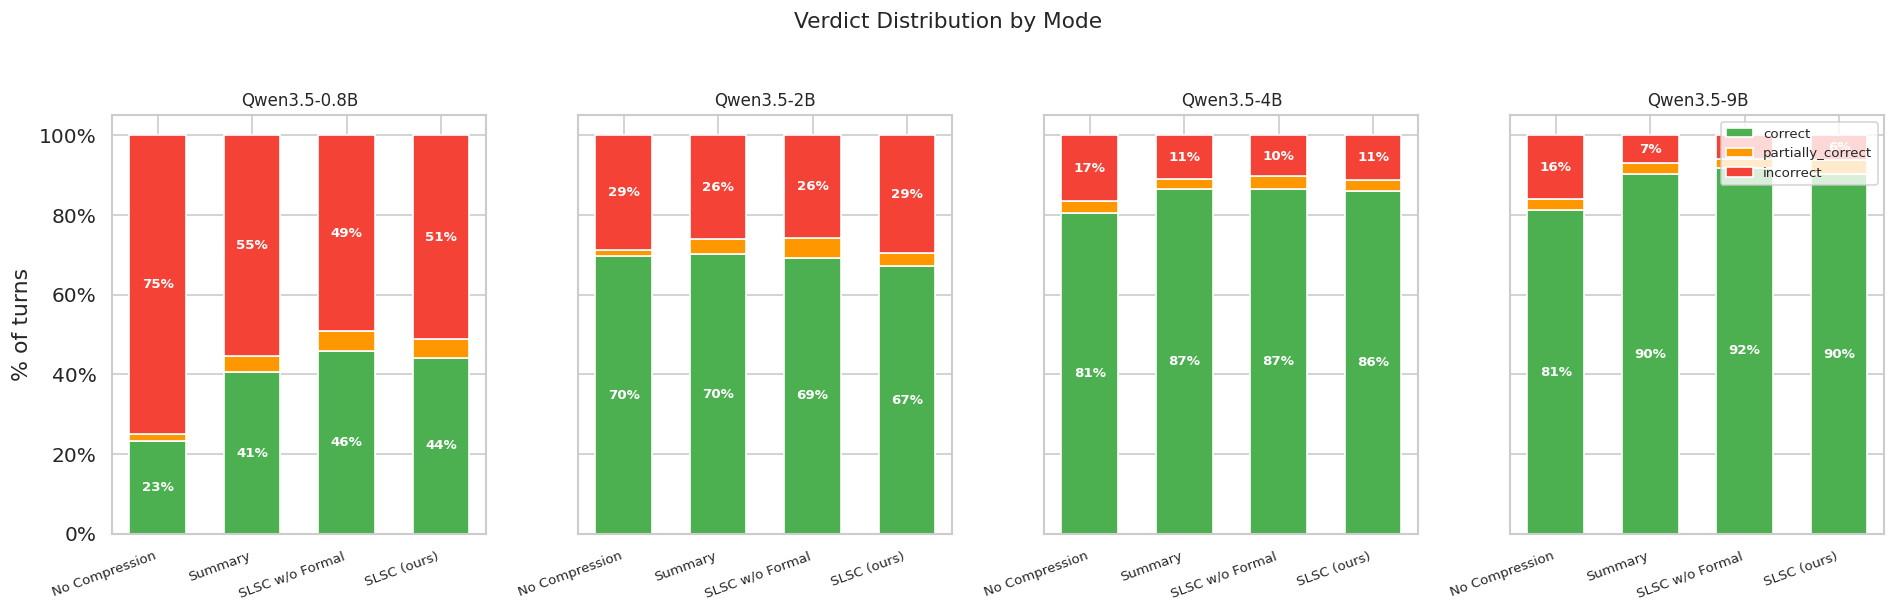
\includegraphics[width=\textwidth]{figures/verdict_distribution.png}
\caption{Per-turn verdict distribution (correct / partially correct / incorrect) for each compression condition, shown separately for each model scale. Stacked bars sum to 100\%. SLSC and SLSC\,w/o Lean~4 shift mass from incorrect to correct relative to No Compression, particularly at smaller scales.}
\label{fig:verdict_dist}
\end{figure*}

\subsection{Token Efficiency Trade-off}
\label{app:token_efficiency}

Figure~\ref{fig:token_efficiency} plots accuracy against average total input tokens (log scale) for all model--condition combinations, illustrating the trade-off between context size and task performance.

\begin{figure*}[t]
\centering
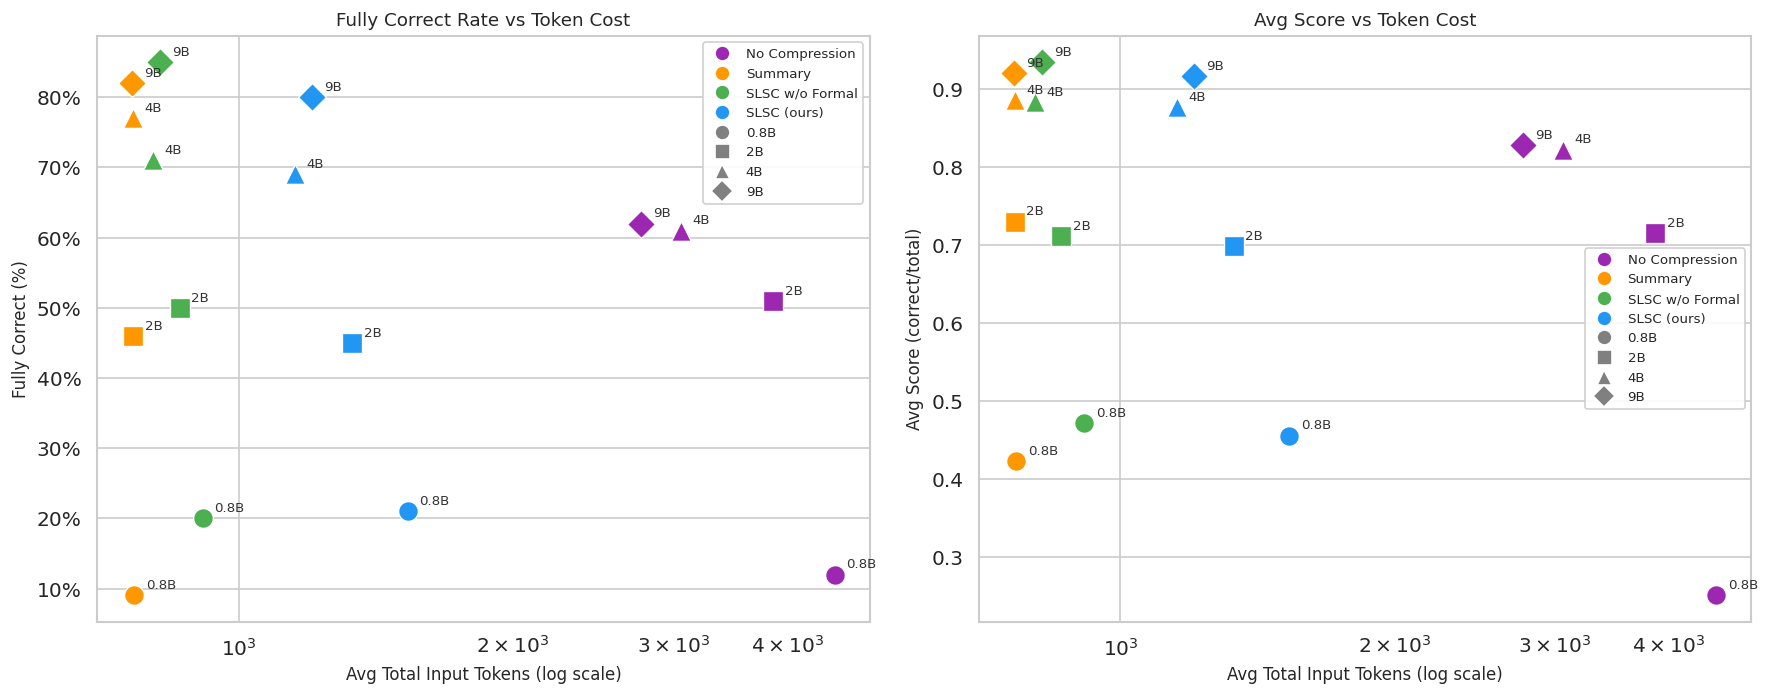
\includegraphics[width=\textwidth]{figures/token_efficiency_scatter.png}
\caption{Token efficiency scatter plot. Each point represents one model--condition pair. \textbf{Left}: Fully Correct Rate (\%) vs.\ average total input tokens (log scale). \textbf{Right}: Average score vs.\ average total input tokens (log scale). Points are colored by compression condition and shaped by model scale. Compression methods consistently achieve higher accuracy at lower token counts than No Compression.}
\label{fig:token_efficiency}
\end{figure*}
